\documentclass{ximera}
\usepackage{epsfig}

\graphicspath{
  {./}
  {figures/}
}

\usepackage{epstopdf}
%\usepackage{ulem}
\usepackage[normalem]{ulem}

\epstopdfsetup{outdir=./}

\usepackage{morewrites}
\makeatletter
\newcommand\subfile[1]{%
\renewcommand{\input}[1]{}%
\begingroup\skip@preamble\otherinput{#1}\endgroup\par\vspace{\topsep}
\let\input\otherinput}
\makeatother

\newcommand{\EXER}{}
\newcommand{\includeexercises}{\EXER\directlua{dofile(kpse.find_file("exercises","lua"))}}

\newenvironment{computerExercise}{\begin{exercise}}{\end{exercise}}

%\newcounter{ccounter}
%\setcounter{ccounter}{1}
%\newcommand{\Chapter}[1]{\setcounter{chapter}{\arabic{ccounter}}\chapter{#1}\addtocounter{ccounter}{1}}

%\newcommand{\section}[1]{\section{#1}\setcounter{thm}{0}\setcounter{equation}{0}}

%\renewcommand{\theequation}{\arabic{chapter}.\arabic{section}.\arabic{equation}}
%\renewcommand{\thefigure}{\arabic{chapter}.\arabic{figure}}
%\renewcommand{\thetable}{\arabic{chapter}.\arabic{table}}

%\newcommand{\Sec}[2]{\section{#1}\markright{\arabic{ccounter}.\arabic{section}.#2}\setcounter{equation}{0}\setcounter{thm}{0}\setcounter{figure}{0}}
  
\newcommand{\Sec}[2]{\section{#1}}

\setcounter{secnumdepth}{2}
%\setcounter{secnumdepth}{1} 

%\newcounter{THM}
%\renewcommand{\theTHM}{\arabic{chapter}.\arabic{section}}

\newcommand{\trademark}{{R\!\!\!\!\!\bigcirc}}
%\newtheorem{exercise}{}

\newcommand{\dfield}{{\sf SlopeField}}

\newcommand{\pplane}{{\sf PhasePlane}}

\newcommand{\PPLANE}{{\sf PHASEPLANE}}

% BADBAD: \newcommand{\Bbb}{\bf}. % Package amsfonts Warning: Obsolete command \Bbb; \mathbb should be used instead.

\newcommand{\R}{\mbox{$\mathbb{R}$}}
\let\C\relax
\newcommand{\C}{\mbox{$\mathbb{C}$}}
\newcommand{\Z}{\mbox{$\mathbb{Z}$}}
\newcommand{\N}{\mbox{$\mathbb{N}$}}
\newcommand{\D}{\mbox{{\bf D}}}

\newcommand{\WW}{\mathcal{W}}

\usepackage{amssymb}
%\newcommand{\qed}{\hfill\mbox{\raggedright$\square$} \vspace{1ex}}
%\newcommand{\proof}{\noindent {\bf Proof:} \hspace{0.1in}}

\newcommand{\setmin}{\;\mbox{--}\;}
\newcommand{\Matlab}{{M\small{AT\-LAB}} }
\newcommand{\Matlabp}{{M\small{AT\-LAB}}}
\newcommand{\computer}{\Matlab Instructions}
\renewcommand{\computer}{M\small{ATLAB} Instructions}
\newcommand{\half}{\mbox{$\frac{1}{2}$}}
\newcommand{\compose}{\raisebox{.15ex}{\mbox{{\scriptsize$\circ$}}}}
\newcommand{\AND}{\quad\mbox{and}\quad}
\newcommand{\vect}[2]{\left(\begin{array}{c} #1_1 \\ \vdots \\
 #1_{#2}\end{array}\right)}
\newcommand{\mattwo}[4]{\left(\begin{array}{rr} #1 & #2\\ #3
&#4\end{array}\right)}
\newcommand{\mattwoc}[4]{\left(\begin{array}{cc} #1 & #2\\ #3
&#4\end{array}\right)}
\newcommand{\vectwo}[2]{\left(\begin{array}{r} #1 \\ #2\end{array}\right)}
\newcommand{\vectwoc}[2]{\left(\begin{array}{c} #1 \\ #2\end{array}\right)}

\newcommand{\ignore}[1]{}


\newcommand{\inv}{^{-1}}
\newcommand{\CC}{{\cal C}}
\newcommand{\CCone}{\CC^1}
\newcommand{\Span}{{\rm span}}
\newcommand{\rank}{{\rm rank}}
\newcommand{\trace}{{\rm tr}}
\newcommand{\RE}{{\rm Re}}
\newcommand{\IM}{{\rm Im}}
\newcommand{\nulls}{{\rm null\;space}}

\newcommand{\dps}{\displaystyle}
\newcommand{\arraystart}{\renewcommand{\arraystretch}{1.8}}
\newcommand{\arrayfinish}{\renewcommand{\arraystretch}{1.2}}
\newcommand{\Start}[1]{\vspace{0.08in}\noindent {\bf Section~\ref{#1}}}
\newcommand{\exer}[1]{\noindent {\bf \ref{#1}}}
\newcommand{\ans}{\textbf{Answer:} }
\newcommand{\matthree}[9]{\left(\begin{array}{rrr} #1 & #2 & #3 \\ #4 & #5 & #6
\\ #7 & #8 & #9\end{array}\right)}
\newcommand{\cvectwo}[2]{\left(\begin{array}{c} #1 \\ #2\end{array}\right)}
\newcommand{\cmatthree}[9]{\left(\begin{array}{ccc} #1 & #2 & #3 \\ #4 & #5 &
#6 \\ #7 & #8 & #9\end{array}\right)}
\newcommand{\vecthree}[3]{\left(\begin{array}{r} #1 \\ #2 \\
#3\end{array}\right)}
\newcommand{\cvecthree}[3]{\left(\begin{array}{c} #1 \\ #2 \\
#3\end{array}\right)}
\newcommand{\cmattwo}[4]{\left(\begin{array}{cc} #1 & #2\\ #3
&#4\end{array}\right)}

\newcommand{\Matrix}[1]{\ensuremath{\left(\begin{array}{rrrrrrrrrrrrrrrrrr} #1 \end{array}\right)}}

\newcommand{\Matrixc}[1]{\ensuremath{\left(\begin{array}{cccccccccccc} #1 \end{array}\right)}}



\renewcommand{\labelenumi}{\theenumi}
\newenvironment{enumeratea}%
{\begingroup
 \renewcommand{\theenumi}{\alph{enumi}}
 \renewcommand{\labelenumi}{(\theenumi)}
 \begin{enumerate}}
 {\end{enumerate}
 \endgroup}

\newcounter{help}
\renewcommand{\thehelp}{\thesection.\arabic{equation}}

%\newenvironment{equation*}%
%{\renewcommand\endequation{\eqno (\theequation)* $$}%
%   \begin{equation}}%
%   {\end{equation}\renewcommand\endequation{\eqno \@eqnnum
%$$\global\@ignoretrue}}

%\input{psfig.tex}

\author{Martin Golubitsky and Michael Dellnitz}

%\newenvironment{matlabEquation}%
%{\renewcommand\endequation{\eqno (\theequation*) $$}%
%   \begin{equation}}%
%   {\end{equation}\renewcommand\endequation{\eqno \@eqnnum
% $$\global\@ignoretrue}}

\newcommand{\soln}{\textbf{Solution:} }
\newcommand{\exercap}[1]{\centerline{Figure~\ref{#1}}}
\newcommand{\exercaptwo}[1]{\centerline{Figure~\ref{#1}a\hspace{2.1in}
Figure~\ref{#1}b}}
\newcommand{\exercapthree}[1]{\centerline{Figure~\ref{#1}a\hspace{1.2in}
Figure~\ref{#1}b\hspace{1.2in}Figure~\ref{#1}c}}
\newcommand{\para}{\hspace{0.4in}}

\usepackage{ifluatex}
\ifluatex
\ifcsname displaysolutions\endcsname%
\else
\renewenvironment{solution}{\suppress}{\endsuppress}
\fi
\else
\renewenvironment{solution}{}{}
\fi

\ifcsname answer\endcsname
\renewcommand{\answer}{}
\fi

%\ifxake
%\newenvironment{matlabEquation}{\begin{equation}}{\end{equation}}
%\else
\newenvironment{matlabEquation}%
{\let\oldtheequation\theequation\renewcommand{\theequation}{\oldtheequation*}\begin{equation}}%
  {\end{equation}\let\theequation\oldtheequation}
%\fi

\makeatother

\newcommand{\RED}[1]{{\color{red}{#1}}} 

\begin{document}
\begin{exercise} \label{c9.1.1}
Consider the Volterra-Lotka equations when $\mu_1,\mu_2>0$, 
$\rho_1,\rho_2 < 0$, and $\sigma_1<0,\sigma_2>0$. Scaling these 
equations leads to the system
\begin{matlabEquation}\label{MATLAB:22}
\begin{array}{rcl}
\dot{x} & = & x(\mu + \rho x -         y)  \\
\dot{y} & = & y(  1 +        x +  \eta y),
\end{array}
\end{matlabEquation}
where $\mu>0$ and $\rho,\eta<0$.  
\begin{itemize}
\item[(a)]  There are four possible equilibria depending on whether $x$ and 
$y$ vanish or not.  Find these equilibria and their type (saddle, sink, 
source or nonhyperbolic).  {\bf Hint:} Use the equations for the equilibrium 
where both coordinates are nonzero 
\[
\mu + \rho x - y = 0 \AND  1 + x +  \eta y = 0
\]
to show that the Jacobian matrix at that equilibrium is:
\[
(df) =\mattwoc{\rho x}{-x}{y}{\eta y}.
\]
\item[(b)]  Set $\rho=-1.5$ and $\eta=-1$ and discuss the phase portraits 
of these equations for different values of $\mu$.  Verify your answer 
using {\pplane}. 
\end{itemize}

\begin{solution}

(a) \ans See Table~\ref{c9.1.1}
\begin{table}[htb]
\begin{center}
\begin{tabular}{|c|c|c|c|}
\hline
& Exists in $1^{st}$ & Jacobian & equilibrium \\
& Quadrant & & type \\
\hline
$e_1 = (0,0)$ & always & $\mattwo{\mu}{0}{0}{1}$ & nodal source \\
\hline
$e_2 = \left(-\frac{\mu}{\rho},0\right)$ & always &
$\cmattwo{-\mu}{\frac{\mu}{\rho}}{0}{1 - \frac{\mu}{\rho}}$ &
saddle point \\
\hline
$e_3 = \left(0,-\frac{1}{\eta}\right)$ & always &
$\cmattwo{\mu + \frac{1}{\eta}}{0}{-\frac{1}{\eta}}{-1}$ &
$\begin{array}{c} \hbox{nodal sink if } \mu < -\frac{1}{\eta} \\
\hbox{saddle node if } \mu = -\frac{1}{\eta} \\
\hbox{saddle if } \mu > -\frac{1}{\eta} \end{array}$ \\
\hline
$\begin{array}{rl} e_4 = & (x_4,y_4) \\
 = & \dps\frac{1}{1 + \rho\eta}(-1 - \mu\eta, \mu - \rho) \end{array}$ 
& $\mu > -\frac{1}{\eta}$ &
$\cmattwo{\rho x_4}{-x_4}{y_4}{\eta y_4}$ & sink \\
\hline
\end{tabular}

\vspace{0.2in}
Table~\ref{c9.1.1}
\end{center}
\end{table}

\soln
Solve
\[
\begin{array}{rcccl}
\dot{x} & = & x(\mu + \rho x - y) & = & 0 \\
\dot{y} & = & y(1 + x + \eta y) & = & 0 \end{array}
\]
There are four solutions:
\[
\begin{array}{lr}
x = y = 0 & (e_1) \\
x \neq 0, y = 0 & (e_2) \\
x = 0, y \neq 0 & (e_3) \\
x \neq 0, y \neq 0 & (e_4) \end{array}
\]

Find the Jacobian matrices at these equilibria, which are shown in
Table~\ref{c9.1.1}.  To find the Jacobian at $e_4$, note that
$\mu + \rho x_4 - y_4 = 0$ and $1 + x_4 + \eta y_4 = 0$.  Therefore,
\[
(dJ)_{e_4} = \cmattwo{\mu + 2\rho x_4 - y_4}{-x_4}{y_4}{1 + x_4 +
2\eta y_4} = \cmattwo{\rho x_4}{-x_4}{y_4}{\eta y_4}.
\]

Use the Jacobian to find the type of each equilibrium.  Since $\mu > 0$,
both eigenvalues of $(dJ)_{e_1}$ are positive, so $e_1$ is a nodal source. 
Since $\det(dJ)_{e_2} < 0$, $e_2$ is a saddle point.  The trace of the
Jacobian at $e_3$ is always negative, so the equilibrium is a saddle if the
determinant is negative, a nodal sink if the determinant is positive, and
a saddle node if the determinant is zero.
For any valid $\rho$ and $\eta$, $\trace(dJ)_{e_4} = \rho x_4 +
\eta y_4 < 0$ and $\det(dJ)_{e_4} = x_4y_4(\rho\eta + 1) > 0$.
Define
\[
D = (\trace(dJ)_{e_4})^2 - 4\det(dJ)_{e_4} =
(\rho x_4 - \eta y_4)^2 - 4x_4y_4.
\]
Therefore, if $D > 0$, then $e_4$ is a spiral sink.  If $D = 0$, then
$e_4$ is an improper nodal sink, and if $D < 0$, then $e_4$ is a nodal
sink.

(b) If $e_4$ exists in the first quadrant, then all initial
populations such that $x > 0$ and $y > 0$ limit on $e_4$ in forward time. 
If $e_4$ does not exist in the first quadrant, then the population limits on
$e_3$, that is, the prey become extinct, and the population of predators
stabilizes at $-\frac{1}{\eta}$.  Figure~\ref{c9.1.1}a shows trajectories
of the system with $\mu = 2$, and Figure~\ref{c9.1.1}b shows trajectories
of the system with $\mu = 0.5$, so that $e_4$ no longer exists in the first
quadrant.

\begin{figure}[htb]
                       \centerline{%
                       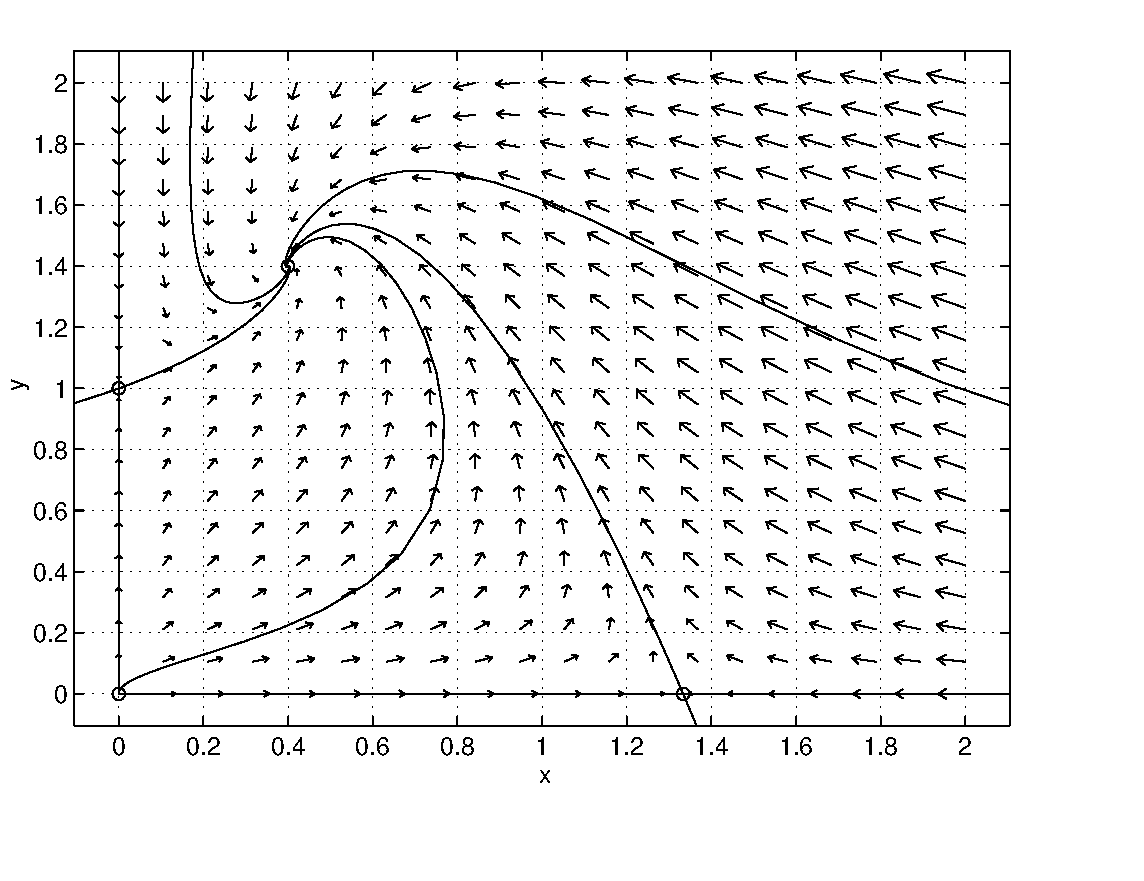
\includegraphics[width=2.75in]{exfigure/9-1-1a.pdf}
                       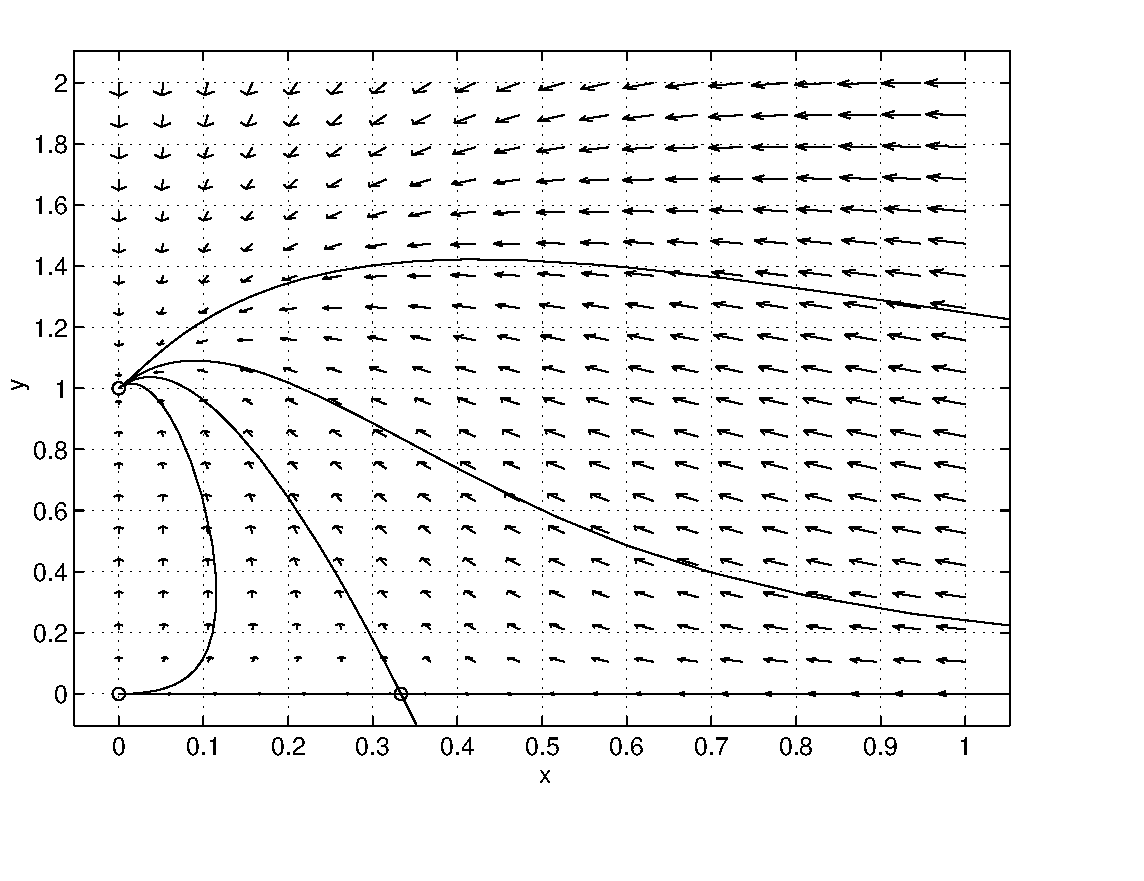
\includegraphics[width=2.75in]{exfigure/9-1-1b.pdf}}
                \exercaptwo{c9.1.1}
\end{figure}

\end{solution}
\end{exercise}
\end{document}
